%------------------------------------------------
\section{Introducción} 
%------------------------------------------------

\subsection{Motivación}

\begin{frame}
	\frametitle{Introducción}
		\begin{block}{Motivación}
			\begin{itemize}
				\item Larga espera.
				\item Optimización del control de paso.
				\item Peatones.
				\item Reducción de consumo.
				\item Contaminación ambiental.
			\end{itemize}
		\end{block}
\end{frame}

\subsection{Antecedentes}

\begin{frame}
\frametitle{Introducción}
\begin{block}{Antecedentes}
	\begin{itemize}
		\item Holanda: Reducción de tiempo entre transiciones % Menos espera teneiendo en cuenta estadistica de acción de los autos entre que aceleran
		\item Brasil: ``SEMINT", utilizando sensores, prioridad, etc % Con paneles solares.
		\item San Juan: Año 2008, utilizando sensores, procesamiento automático
	\end{itemize}
\end{block}
\end{frame}

%------------------------------------------------
\section{Modelado y abstracción}
%------------------------------------------------

\begin{frame}
\frametitle{Modelado y abstracción}
\begin{block}{Intersección entre dos avenidas}
	\begin{itemize}
		\item Sensores de proximidad que simulan la presencia de autos en cada tramo.
		\item Tareas que controlan el comportamiento de cada semáforo.
		\item La intersección es el recurso compartido entre todas las tareas.
		\item Los accesos deben serializarse.
		\item Primitivas de sincronización (mutexes).
	\end{itemize}
\end{block}
\end{frame}

\subsection{Ningún tramo activo}
\begin{figure}[htbp]
	\centering
	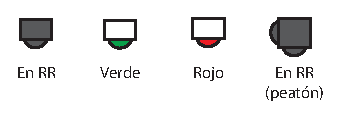
\includegraphics[width=0.8\textwidth]{diagramas/leyenda.eps}
\end{figure}
\begin{figure}[htbp]
	\centering
	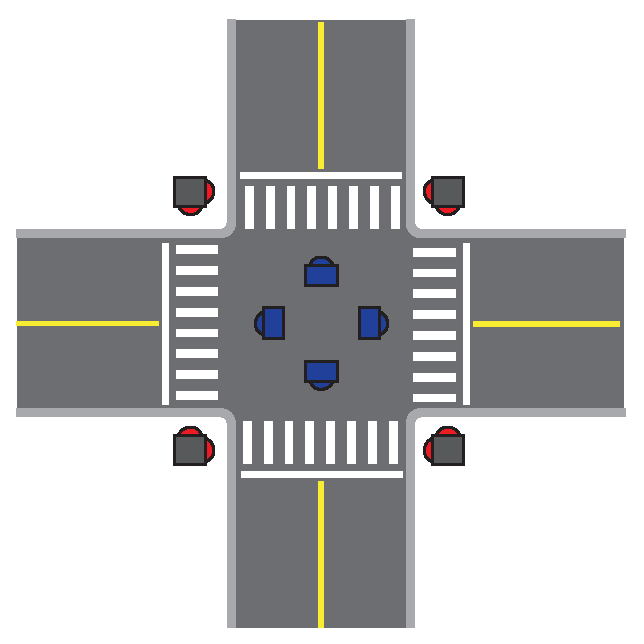
\includegraphics[width=0.8\textwidth]{diagramas/ningun-activo.eps}
	\caption{Esquema con todos los tramo inactivos.}
\end{figure}

\subsection{Un tramo activo}
\begin{figure}[htbp]
	\centering
	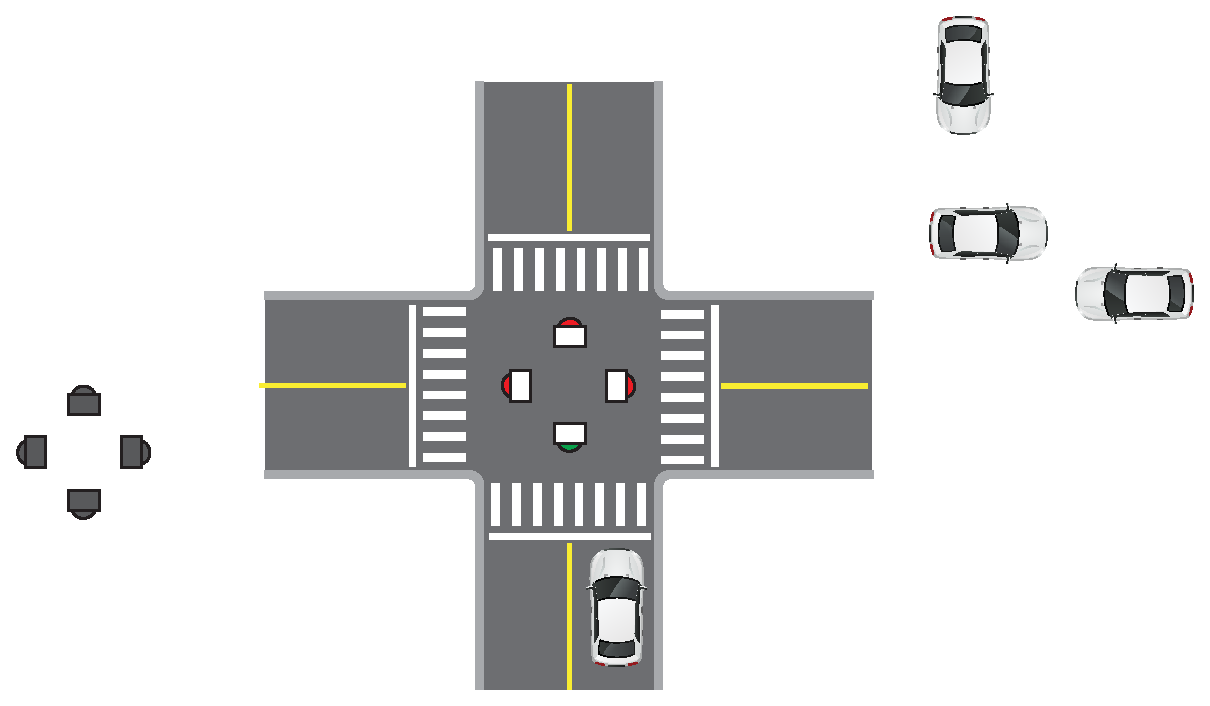
\includegraphics[width=1.2\textwidth]{diagramas/un-activo.eps}
	\caption{Esquema con un solo tramo activo.}
\end{figure}

\subsection{Más de un tramo activo}
\begin{figure}[htbp]
	\centering
	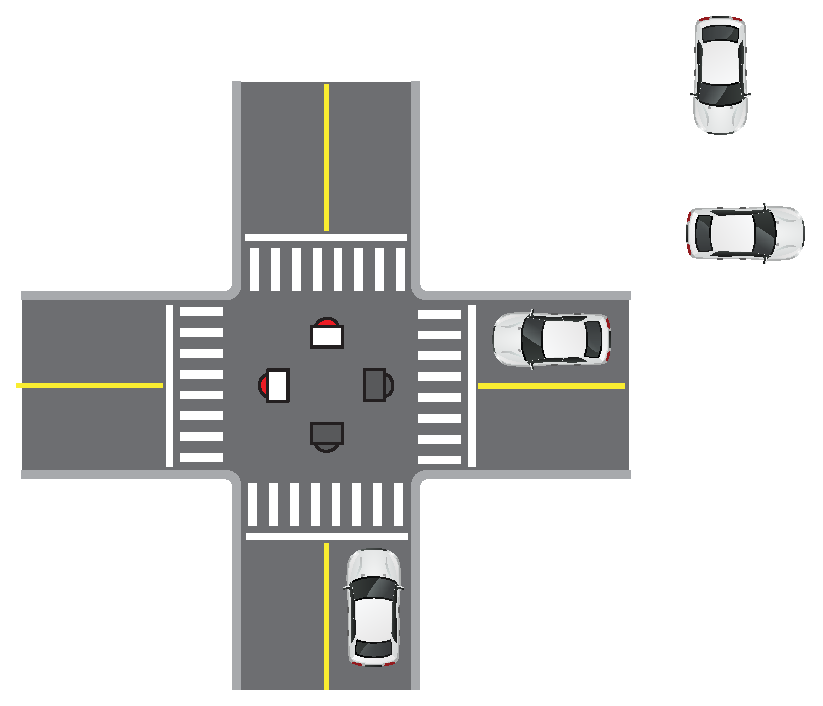
\includegraphics[width=0.9\textwidth]{diagramas/dos-activos.eps}
	\caption{Esquema con más de un tramo activo.}
\end{figure}

\subsection{Todos los tramos activos}
\begin{figure}[htbp]
	\centering
	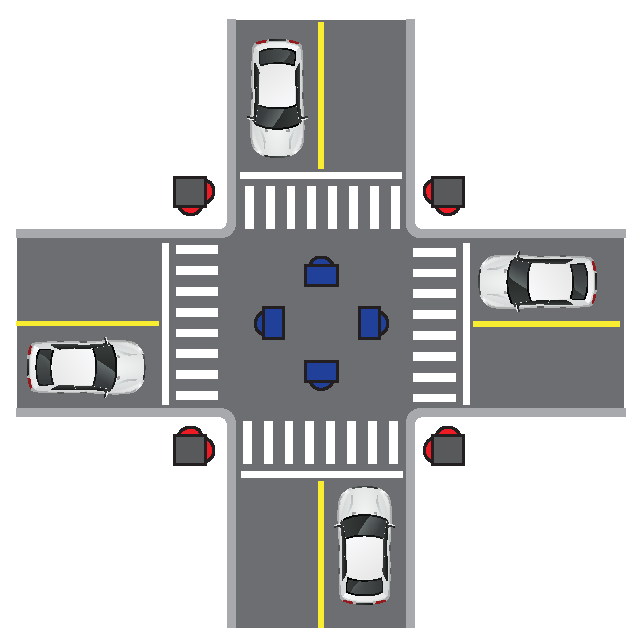
\includegraphics[width=0.5\textwidth]{diagramas/todos-activos.eps}
	\caption{Esquema con todos los tramos activos.}
\end{figure}

\subsection{Peatones}
\begin{figure}[htbp]
	\centering
	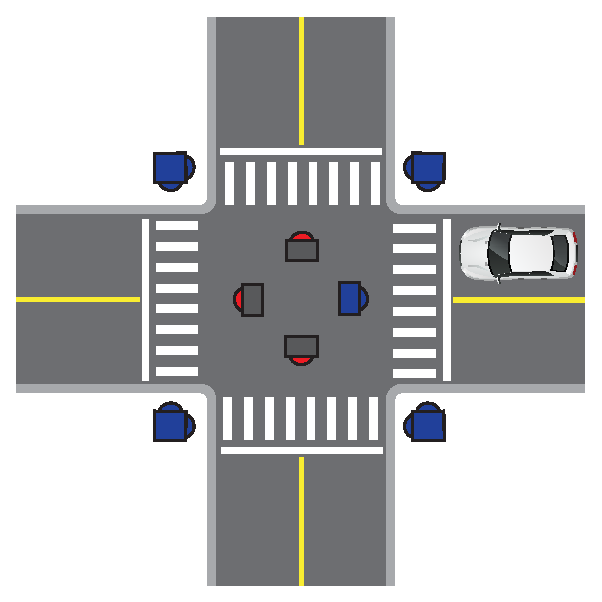
\includegraphics[width=1\textwidth]{diagramas/peaton-auto.eps}
	\caption{Esquema de un tramo activo con peatones.}
\end{figure}

%------------------------------------------------
\section{Implementaciones}
%------------------------------------------------

\subsection{Primera implementación}

\begin{frame}
\frametitle{Implementaciones}
\begin{block}{Única sección crítica con una clase controlador.}
	\begin{itemize}
		\item Planificación a cargo de una tarea de alta prioridad.
		\item Diferentes prioridades estáticas.
		\item Modelo productor-consumidor.
		\item Poca escalabilidad.
		\item Dificultad para agregar un control sobre los peatones.
		%\item Debido a las prioridades estáticas, cuando todos los tramos están inactivos, no se puede realizar el Round-Robin%
	\end{itemize}
\end{block}
\end{frame}

\subsection{Segunda implementación}
\begin{frame}
\frametitle{Implementaciones}
\begin{block}{Única sección crítica sin una clase controlador.}
	\begin{itemize}
		\item Planificación a cargo del scheduler de FreeRTOS.
		\item Prioridades variables a lo largo del tiempo.
		\item Escalabilidad.
		\item Permite agregar una tarea que controle la circulación de los peatones.
		\item Grave problema respecto al cambio de prioridad sobre tareas bloqueadas.
	\end{itemize}
\end{block}
\end{frame}

\subsection{Problemas}
\begin{frame}
\frametitle{Problemas}
\begin{block}{}
	\begin{itemize}
		\item
	\end{itemize}
\end{block}
\end{frame}

\subsection{Tercera Implemetanción}
\begin{frame}
\frametitle{Implementaciones}
\begin{block}{Múltiples secciones críticas y sistema basado en turnos.}
	\begin{itemize}
		\item Cada semáforo se duerme en su propio mutex.
		\item No se realizan cambios de prioridades sobre tareas dormidas.
		\item Prioridades estáticas.
		\item Escalabilidad.
		\item Permite fácilmente agregar el control del peatón como si fuese otro semáforo más.
		\item Modelo \emph{passing the baton}.
	\end{itemize}
\end{block}
\end{frame}

%------------------------------------------------
\section{Conclusiones}
%------------------------------------------------

\subsection{Conclusiones}
\begin{frame}
	\begin{block}{Conclusiones}
	\end{block}
\end{frame}